\documentclass[12pt,oneside]{amsbook}
\usepackage[utf8]{inputenc}
\usepackage[
backend=bibtex,
sorting=ynt
]{biblatex}
\usepackage{import}
\usepackage{graphicx}
\addbibresource{TheBib.bib} %Imports bibliography file



\newcommand{\eps}{\varepsilon^t_i}
\newcommand{\bet}{\beta^t}
\newcommand{\zet}{z^t}
\newcommand{\dos}{{t + \tau}}
\newcommand{\deps}{\varepsilon^\dos_i}
\newcommand{\teps}{\varepsilon^{t,\dos}_i}
\newcommand{\et}{\textit{et. al. }}





\begin{document}
\frontmatter
\title[]{Distance Invariant Foreclosure Contagion}
\author{Tynan Flawn Sailor Daly}
\address{Department of Economics\\Bates College\\Lewiston, ME 04240
\begin{center}

\includegraphics{imgres.jpg}
\end{center}
}

\maketitle


\thispagestyle{empty}
% THESIS COVER PAGE

% Choose Honors/Senior and Arts/Science below as appropriate.

\vspace*{4cm} 
% LaTeX will remove blank space at the start or end of a page,
%   but the asterisk prevents this.

\centerline{\LARGE \textbf{Distance Invariant Foreclosure Contagion}}
%\centerline{\LARGE \textbf{Topology and Stuff}}
\bigskip\bigskip

%\centerline{\Large  A Senior Thesis}
\medskip
\centerline{\Large Presented to the Department of Economics}
\medskip
\centerline{\Large Bates College}
\medskip
\centerline{\Large in partial fulfillment of the requirements for the}
\medskip
\centerline{\Large Degree of Bachelor of Arts}
%\centerline{\Large Degree of Bachelor of Science}
\medskip
\centerline{\Large by}
\medskip
\centerline{\Large Tynan Flawn Sailor Daly}
\medskip
\centerline{\Large Lewiston, Maine}
\medskip
\centerline{\Large April, 2015}

\newpage


\setcounter{page}{2}


\thispagestyle{empty}

\clearpage
\import{}{ack.tex}

\setcounter{tocdepth}{2}
\tableofcontents
 
\listoffigures
 
\mainmatter
\section{Introduction}\label{intro}
In the lead up to and throughout the 2008 financial crisis, real estate markets across the country experienced wave upon wave of unexpected foreclosures on a scale not seen in decades. Due in large part to the nature of mortgage securitization, the bursting of the housing bubble and subsequent decline in home prices have negatively affected almost every major market in the United States. 

	In light of recent events, the dynamic interaction of housing prices and foreclosures has become a popular topic for both theoretical and empirical literature. While this interaction has important macroeconomic implications, much of the literature surrounding the topic attempts to answer using micro level analysis. We feel that while such contributions are meaningful, they lack a benchmark figure to which they may be compared. We contribute to the field by estimating the national foreclosure contagion discount.
	
On average, we find that an increase in one foreclosure per ten thousand homes results in a median home price decrease of $-0.99171\%$. We also find that this affect is increased for homes in areas with relatively low levels of foreclosure. 

	Our results have wide ranging policy implications. A recent renewal of interest in foreclosure relief efforts has opened new avenues for funding. In order to maximize the impact of such initiatives, foreclosure relief should be targeted to those markets which suffer disproportionately. On a micro level, alleviating housing markets disproportionately affected by foreclosure activity can reduce crime. On a macro level, housing prices have been shown to be an important factor in economic downturns\cite{paul}. As a result, we feel that adequate foreclosure relief efforts may potentially dampen business cycle contractions.

\section{Literature}\label{sec:lit}
\subsection{The Foreclosure Discount}
In the face of adequate characteristic controls, the literature is apt to opt for the existence of a liquidity discount. Faced with various holding costs associated with home ownership, lenders in possession of repossessed home may choose to accept a lower sale price in order to achieve a faster sale. Classical theory, however, would suggest that this would result in buyers engaging in arbitrage and thus reducing the time under sale of foreclosed homes. A brief survey of the literature and an analysis of our data quickly disprove this intuition. 

	In order to explain this discrepancy, theorists have proposed that foreclosure signals a decline in property condition \cite{Foote}. Borrowers undergoing foreclosure are likely in financial distress. As a result, it seems plausible that they may forgo normal house maintenance payments in order to meet their current debt obligations. This results in a decline in either actual or perceived property values. Recent research has shown that those homes in foreclosure perceived to be of less than average quality face a higher foreclosure discount \cite{Frame}. 
	
The cause of this decline in property condition is twofold. Typically, the initiation of foreclosure proceedings results in the eviction of the occupants which leaves the home vacant for the duration of the legal process. Vacant properties accumulate distress at a higher rate than non-vacant properties either through the absence of maintenance or the attraction of criminal behavior. Additionally, homeowners facing eviction have been known to reduce home values by intentionally damaging the soon to be repossessed property. 

This channel can be thought of as a lemon discount. Because potential home buyers face an asymmetry of information when compared to sellers, they may use a home’s foreclosure status as a signal that the property was or in currently in a distressed state. While legal protections exist in many states for lemon homes, the potential losses associated with such a large purchase may be inhibitory. 

\subsection{Channels of Contagion}
Although the link between foreclosure events and home price declines has been long established, research into foreclosure as mechanism of contagion was extraordinarily thin before the market crash of 2008. Building off the some of the work summarized by Frame, Lee identified three possible channels of contagion; blight, valuation, and supply \cite{Lee}. 

	Blight functions similarly to the lemon mechanism discussed above. Because foreclosure have been shown to attract vandalism and increase crime, blight from properties under foreclosure may spread to neighboring residences \cite{Crime}. Because many communities rely on property taxes for services, this blight may extend to nearby institutions. Housing appraisals commonly incorporate comparative valuation techniques, and so homes with a foreclosure discount may lower nearby home prices \cite{Lee}. Additionally, foreclosures concentrated in a geographical area can increase the housing stock in face thus lowering prices, which may be accelerated by seller urgency.  
	
Interestingly, it appears that the impact of a foreclosure event is also dependent on the loan originator and structure. Immergluck and Smith find that foreclosures with sub-prime or Alt-A mortgages produce the greatest degree of contagion \cite{Immer}. Conventional or prime mortgages produce much more modest contagion and mortgages with government guarantees produce almost no contagion effect. Naturally, one would hope to find further research into this topic, however, this literature appears to be remarkably sparse.

	While it appears that foreclosure are contagious, the effect of a single foreclosure event decreases non-linearly with both distance and time. Been demonstrated that, although contagious, foreclosure discounts dissipate around the 1.6 miles from a foreclosure event \cite{Been}. These effects also decrease over time. Lin, Rosenblatt, and Yao have shown the foreclosure event contagion can be as high as -8.7\% in the Chicago metropolitan area \cite{Spillover}. This research has been corroborated by Campbell, Giglio, and Pathak, which found a foreclosure discount of 7-9\% for nearby non-foreclosed homes \cite{Forces}. Although these results are incredible, they are done using hedonic estimation techniques. In a follow up study, Harding, Rosenblatt and Yao used repeat homes samples an alternative to hedonic methods and found a discount of 1\% \cite{Chi}. This discrepancy highlights the importance of controlling for neighborhood and home characteristics. 
	
	Until recently, discussion of strategic default has been largely absent from the research. Home owners have the equivalent of a put option by simply allowing a creditor to take possession of their house. In their seminal 2008 paper, Foote, Gerardi, and Willen find that only ten percent of borrowers with negative equity experience any type of repossession \cite{Foote}. Given that borrowers are always financially better off walking away from negative equity positions, it seems odd that so few home owners chose to continue servicing their debt obligations simply because they want to. In response, Goodstein, Hanouna, Ramirez, and Stahel conclude homeowners are reluctant to exercise strategic default options because they lack relevant information. They further find areas with at least one strategic default to increase probability of subsequent defaults by up to 16.5\% \cite{Strat}.
	
	They present several possible explanations for this relationship. Because it rarely utilized, borrower information surround strategic default is limited. It follows that those who chose to exercise this option can help interested parties navigate the legal and financial default process. Secondly, concentrations of strategic defaults can normalize this behavior and thus remove any associated moral hazard. Finally, mass disruption can sever social ties and thus reduce the inclination of negative equity borrowers to continue making payments. These causal links are important to explain in remedying some of the discrepancies found in the traditional literature.


\section{Methodology}\label{sec:method}
\indent Following the existing literature, we adopt a hedonic regression techniques to estimate foreclosure contagion.\footnote{Our theoretical understanding of hedonic regression techniques are based off of \cite{Hedonic} \cite{Monson} \cite{Diwert}. } For this method to hold, we assume that housing goods are, at their root, a bundle of characteristics. This bundle may consist of an array of variables, some of which are quantifiable, such as lot size or square footage, while others are dependent on consumer preferences, such as architectural style. 

\subsection{Econometric Theory}\label{sec:metrics}
The hedonic regression model defines the price $p$ of property $i$ at time $t$ to be a function of a finite number of characteristics $K$ measured as $z_{i,K}^t$, which we permit to be either a quantitative or binary variable. For $T+1$ time periods, the price at time $t$ where $0\leq t \leq T$, the price is
\begin{align}
p^t_{i,K} &= f(z_{i,1}^t, \dots,  z_{i,K-1}^t, z_{i,k}^t, \eps)
\end{align}
where $t \in [0, T]$. As de Haan and Diewert point out, price of a home is equal to the sum of price of characteristic structure and the land \cite{Hedonic}. Land valuation data, however, is difficult to obtain and linear hedonic estimation techniques depend on a lack of omitted variable bias. Thus we use the log-linear model 
\begin{align}
 p^t_{i} & = e^{ \bet_0 + \sum^K_{k=1}\beta^t_k \zet_{i,k} + \eps}\\
\ln (p^t_{i}) & = \bet_0 + \sum^K_{k=1}\beta^t_k \zet_{i,k} + \eps \label{eq:time}
\end{align}
where $\bet_0$ is the intercept term and $\bet_k$ is the parameter coefficient we are trying to determine. 

    We introduce a further simplifying assumption by assuming that $\bet_k$ is constant over a sort time horizon. Although it is clear that parameters for housing stock change over time, these changes take place gradually. Therefore, we assume $\bet_k$ to be constant for time periods less than twenty-four months. With this assumption, the model in (\ref{eq:time}) is now 
\begin{align}
\ln (p^t_{i}) & = \bet_0 + \sum^K_{k=1}\beta_k \zet_{i,k} + \eps.\label{eq:bet_time}
\end{align}

    Since we know the sale price and characteristics for each sample $S(t)$ the sample size $N(t)$, where $t \in [0, T]$, we can further constrain (\ref{eq:bet_time}) by pooled estimation if we include a time dummy variable. This is called the time dummy variable hedonic model and is given as 
\begin{align}
\ln (p^t_{i}) & = \beta_0 + \sum^T_{\tau=1} \delta^\tau D^\tau_i+ \sum^K_{k=1}\beta_k \zet_{i,k} + \eps \label{eq:time_dummy_basic}
\end{align}

where the time dummy $D^\tau_i = 1$ if the observation originates from $\tau$ and is otherwise $0$. We also discount the base period, thus if $t=1$ and $\tau=1$, then $D^\tau_i = 0$. Since the a pooled regression preserves degrees of freedom when working with panel data, the estimated coefficients $\hat{\beta}_k$ will have a lower standard error than $\hat{\beta}^t_k$ and thus increases the efficiency of our model. It should be noted that de Haan and Diewert are quick to point out that this relies on a fixed set of parameters, and so we will lose descriptive power of the set of parameters when $z_k^0 = z_k^t$. Our data, however, it at the monthly frequency, which we feel is a small enough time period such that only minor adaptations in housing characteristics may occur. Although we feel justified in assuming constant parameters, we will consider cases where $\hat{\beta}^t_k$ is either fixed or variable. 

The time dummy variable hedonic model also benefits from larger time samples. As $T$ increases, the previously discussed pooled efficiency increases. Considering our sample contains a maximum of 226 months, which is the largest time sample we have yet been able to discover, our model should be able to provide the most efficient estimates of the literature. 

\subsection{The Model}\label{sec:model}
We begin by modifying our baseline model to include a measure of foreclosure for a given geographic region. Let $N_i^t$ be the ration of homes per ten-thousand which are in foreclosure in region $i$. After incorporating the new term into (\ref{eq:time}) and taking the natural log, our equation for the price of the first sale at time $t$ is 
\begin{align}
\ln (p^t_{i}) & = \beta^t_0 + \sum^K_{k=1}\beta^t_k \zet_{i,k} + \alpha N_i^t +  \eps.
\end{align}

Although we utilize a hedonic regression, we must be careful to not violate its key assumption that the parameter characteristics are well specified. If we fail to include relevant explanatory characteristic variables, our model will suffer from an omitted variable bias. This problem in compounded because the bias will also emerge in the predicted prices estimated from our characteristic parameters. 

Several studies (\cite{Chi} \cite{Spillover} \cite{Boston} \cite{Strat}) have attempted to resolve this issue by using only repeat home sales in their samples. Repeat home sale data is difficult to obtain. Each study either collected it by hand from local records or purchased it from an on-line database. Given the monetary, temporal, and physical constraints of our research, we were unable to obtain similar samples. Thus our model for a sale at time $\dos$ is 
\begin{align}
\ln (p^t_{i}) & = \beta^\dos_0 + \sum^K_{k=1}\beta^\dos_k z^\dos_{i,k} + \alpha N_i^\dos + \deps \label{eq:fuck}
\end{align}
where $\tau \in \mathbb{N}$.

Homes are heterogeneous to the point that we consider them unique goods. Given that no two homes are identical and that consumer preference may change when deciding between homes, we feel justified to assume that both characteristics and their coefficients change not only between buyer, but also within a buyer choosing to buy a home. This makes proper specification of our model exceedingly difficult. 

Thus in order to make our model well specified, we must introduce additional assumptions about housing markets. We assume that given a sufficiently large area, in this case a Z.I.P.+4 code, housing stock will reach can approximate net substitutes of one another. We justify this with two reasons. The first is that the price of a house acts as an information signal for the \textit{norm} coefficient parameters. If we assume that the characteristic parameters change between homes for each buyer, utility maximization becomes computationally complex. In order to constrain the solution space, they relinquish their individual preference to group norms. 

Conversely, our second reason assumes a relatively stable parameter coefficients vector. If a buyer with well defined tastes could have maximized their utility by purchasing home $a$, but is unable to do so, then they can maximize their utility by purchasing a home which is the nearest linear approximation to $a$. If these conditions hold, then $\bet_k = \beta_k^{t+\tau}$ where $\tau \in \mathbb{N}$. Thus our model for the price difference between time $t$ and $\dos$ is
\begin{align}
\ln (p^\dos_i /p^t_{i}  ) & =  \alpha ( N_i^\dos - N_i^t ) + \teps \label{eq:fdiff}
\end{align}
where is $( N_i^\dos - N_i^t )$ is the difference in the foreclosure rate in time $\dos$ with respect to time $t$ and the parameter coefficient $\alpha$ is an estimate of the foreclosure discount. The error term of equation \ref{eq:fdiff} is the difference between $\eps$ and $\deps$. So long as $( N_i^\dos - N_i^t )$ is not correlated with the error term, it will be unbiased. Likewise, if the error term is correlated with any characteristic, our estimation will be biased. 

Although it may be easy to test most OLS models for endogeneity, some of our characteristics are fundamentally unobservable. This in unfortunate, however, we are not aware of any way to test for this. Furthermore, if an unobservable characteristic is endogenous, then the literature as a whole would behave similarly. Thus we proceed to finish deriving our baseline model. 

To finish, we reintroduce the constant terms to the equation. Agreeing with \cite{Chi}, we retain the difference of the intercepts. This allows us to estimate the change in the underlying price structure of a housing market. This is relevant to the model because it allows us to capture both deflating and inflating bubbles in our regression. Because our sample spans the Subprime Mortgage Crisis, regressions which do not control for changes in the underlying price level will suffer from an omitted variable bias. Thus, we control for this by including the term $(\beta^\dos - \bet)$, which yields equation~\ref{eq:baseline}.
\begin{align}
\ln (p^t_{i} / p^\dos_i) & = (\beta^\dos - \bet) + \alpha ( N_i^\dos - N_i^t ) + \teps \label{eq:baseline}
\end{align}

\section{Data}
Although we have a tractable model, choosing a sample for this type of regression can be challenging. Much of the literature surrounding housing markets restricts their analysis to one particular geographic area. While we view this as a limitation, there are several significant benefits to analyzing the impact of foreclosure events.

As we have discussed previously, housing markets are highly differentiated. Even within a given metropolitan area, the neighborhood quality varies considerably, but even deciding what constitutes neighborhood quality poses problems. Beyond matters of individual convenience, such as proximity to areas of interest, the unobservable set of preferences can be broad. Buyers may prefer better access to public goods, such as public education, even if it meant sacrificing relative neighborhood safety, or they might value the `hipness' of one geographic area over. 

While these are important considerations for individual consumers, we forgo their inclusion in our analysis. There is a considerably body of research (\cite{Crime} \cite{Immer} \cite{Leo}) investigating relationship between perceived neighborhood quality and foreclosure events, which raises concerns about possible endogeneity with our foreclosure variables. This may have the unintended consequence of introducing an omitted variable bias into our results. Regardless, we feel the econometric justification pertaining to Equation~\ref{eq:fdiff}. Additionally, we feel the spatial scope of our data will largely filter out the variation of characteristic preferences and so chose to focus on quantitative price and foreclosure measurements. 

The variables we do choose to incorporate into our analysis consists of median home prices, foreclosures per ten thousand homes, and percentage of homes in foreclosure for the ZIP+4 codes comprising the twenty Metropolitan Statistical Areas (MSAs) corresponding to the S\&P/Case-Schiller 20-City Composite Home Price Index.

In a departure for the literature, we do not chose to exclusively employ repeat home sales in our sample for a number of reasons. Because we are interested in determining the temporal behavior of foreclosure contagion and so chose a broader unit of distance, we feel that our sample approximates the repeat home sales filtering method. Additionally, these filtering techniques exclude newer homes, which incidentally were disproportionately financed through the use of subprime loans.\footnote{This particular issue was pointed out by Harding \et \cite{Chi} . } 

Because the necessary data was not widely available, we chose to assemble it ourselves using an Automated Programming Interface provided by Quandl Inc.\footnote{Full documentation for this procedure can be found in the supplementary materials. Per Quandl's terms of use, however, we do not disclose our authentication token} Since we had no \textit{a priori} knowledge of data availability, we employed an uniformed search algorithm to parse all US ZIP codes. All samples consist of monthly observations ranging from twenty-six to two-hundred and twenty six observations starting in April, 1996 and terminating is February 2015. We then screened samples for balance and selected observations corresponding the the 20 MSAs.\footnote{ZIP codes corresponding to the Case-Schiller index can be found at \cite{Case}.}

Home prices are grouped according the number of bedrooms a home posses. We collected data for homes with one, two, three, four, and five or more bedrooms as well as their weighted average. We use the weighted average for our analysis and incorporate bedroom partitioned data for robustness checks. Although the use of weighted data can result in heterogeneity, we feel they this affect does not persist when aggregated across the MSAs. Price variable are in median US dollars and deflated using a non-fixed reference point. 

Foreclosure measurements are either given as a ratio of foreclosures per ten thousand homes or as a percentage of all homes in a ZIP code. We opt to use the ratio during our primary analysis because it is both more sensitive to single foreclosure events and controls for the number of homes in a given ZIP code. Descriptive Statistics for all variables can be found in Appendix \ref{app:B}. 

	The nature of pre-bubble housing market performance also bears mention. Housing markets which are insulated from the housing bubble, such as St. Louise, are generally more highly influenced by the local economic climate \cite{Impact}. Analysis of foreclosure events done on such housing markets produces results with higher confidence levels. Alternatively, using housing markets which experienced relatively strong performance during the housing boom, such as Chicago and Los Angeles, may provide deeper insight in to the true nature of the foreclosure home price relationship. Housing markets which have historically experienced higher exposure have also been those most highly studied. We feel that this allows our research to be more thoroughly compared to past studies. We choose to use both types of markets in our research because \textit{a priori} filtering in this method is likely to bias our results in unknown ways. 



\section{Results}
    In order to conduct any regressions, we need to specify an interval for $\tau$ to range over. We chose a this interval to be twelve months, $\tau \in \{1, 2, \dots, 12\}$, for several reasons. In order for our theoretical model (\ref{eq:baseline}) to hold, the characteristic vectors and their parameters must remain constant. We feel that twelve months is an appropriate measure as it becomes increasingly difficult for consumer make precise plans past this point. Additionally, Zillow deflates home prices by using a backwards looking reference window of twelve months. This important because consumers do not measure home prices in real terms. Instead, they consider the home prices with regard to their semi-real, or partially controlled, performance. \\
    
\subsection{Linear Specification}    
\indent While previous research has focused on the behavior of individual MSA housing markets, we are interested the fundamental, or general, value of foreclosure contagion. Thus we estimate the parameters of Equation~\ref{eq:baseline} jointly. In order to interpret our estimated coefficients, we exponentiate and subtract one to find the percent change in the median home price rusting from a one one-thousandth increase in the number of foreclosed homes per ten thousand in period $t + \tau$ . 
\begin{align*}
\Delta p_i^{t + \tau} = e^{\alpha (\Delta N_i^{t + \tau})} -1
\end{align*}
    The contagion discount for each time period can be found in Table X of the appendix. \\
\begin{figure}\label{fig:avg}
\centering

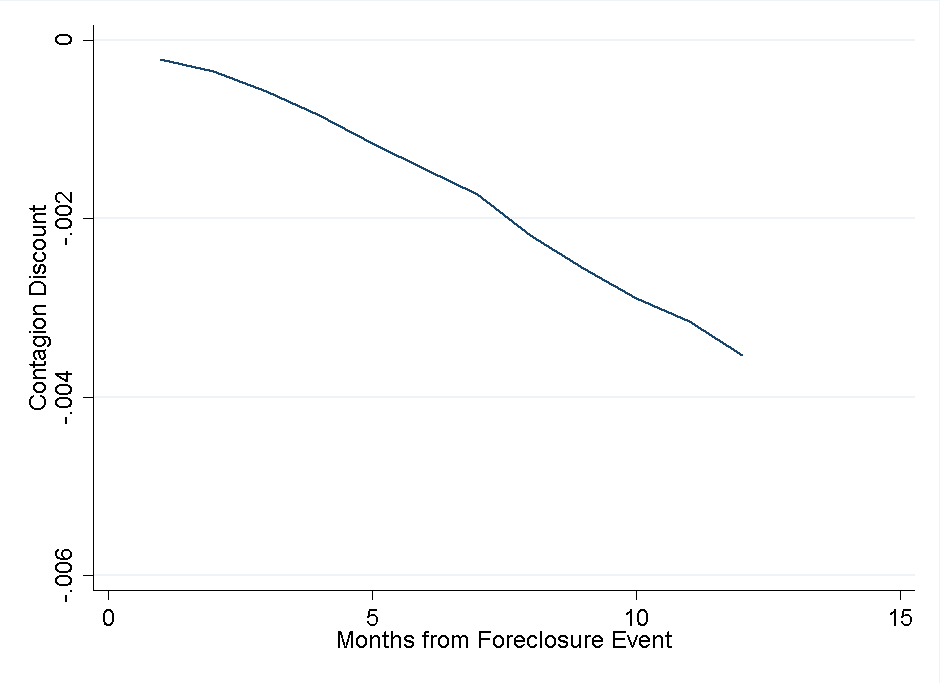
\includegraphics[width=\textwidth]{20MSA_solo.png}
\caption{\tiny Average contagion affect. The figure displays the estimated discount originating from one foreclosure event per ten thousand home in a ZIP code. The time period ranges from $t+1$ to $t+12$. }


\end{figure}
    Figure~\ref{fig:avg} displays the cumulative average affect of foreclosure contagion over a ranger of one year. We estimate the foreclosure discount to be approximately a $-.0056829$ percent decrease in the median home value. When compared to the literature, our results may appear to be economically insignificant. However, because our analysis employs ratios rather than spatial measures, we require further context. Given that distance from a foreclosure event has been shown to be a substantial factor and since we control for it by aggregating over a relatively large geographical area, a smaller coefficient is to be expected. 
    
    However, this does not mean that our results are economically insignificant. During the housing crisis, some markets recorded as many as 3,500 foreclosure events per month \cite{news}. Harding \et have also shown that the discount contagiousness has a decreasing marginal effect \cite{Chi}. In light of the fact the maximum change in the foreclosure ratio 
    
    We explore the possibility of a contagion discount with decreasing marginal returns by partitioning the data set in to quartiles of the foreclosure ratio. However, because periods of high foreclosure rates are rare in our sample, we hypothesize that regressions with standard errors will be heteroskedastic. To correct for this, we estimate our new parameters robustly with heteroskedasticity-consistent standard errors.

\import{Regs/}{results1.tex}

\begin{figure}\label{graph:lin_quart}
\centering
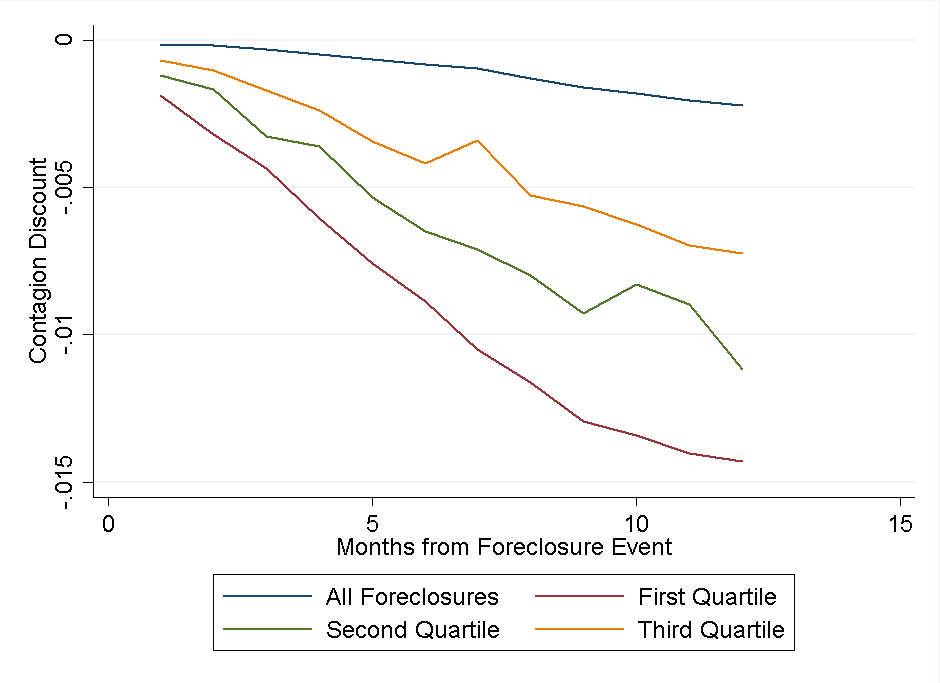
\includegraphics[width=\textwidth]{20MSA_linquart.png}
\caption{\tiny Average contagion affect by quartile. The figure displays the estimated discount with heteroskedasticity-consistent standard errors originating from one foreclosure event per ten thousand home in a ZIP code by quartile. The time period ranges from $t+1$ to $t+12$. }
\end{figure}

Figure~\ref{graph:lin_quart} displays estimated foreclosure discount over time. Table~\ref{table:basic_results} provides a summary of the average foreclosure discount experienced over twelve months. As we can see, the foreclosure discount exhibits significant degree of diminishing marginal returns. This is consistent with the current literature. 

\subsection{The Quadratic Model}
Interestingly, they also appear to behave non-linearly with time. However, this creates a problem for our analysis. We estimated our parameters linearly, but since they display non-linear behavior, it seems likely that our analysis suffers from an omitted variable bias. The model presented in equation~\ref{eq:baseline} was derived from a model assuming a maximum of one additional foreclosure, but is not reflective of reality. 

To correct our model, we introduce a non-linear term of foreclosure rates to  equation~\ref{eq:fuck}. After we rederive, our non-linear model is 

\begin{align}
\ln (p^t_{i} / p^\dos_i) & = (\beta^\dos - \bet) + \alpha_1 ( N_i^\dos - N_i^t ) + \alpha_2 M + \teps \label{eq:nonlin}
\end{align} 
where $M =  (N_i^\dos)^2 - (N_i^t )^2$. 

\import{Regs/}{Simple_Qt_results.tex}
 The average foreclosure discount is presented in Table~\ref{table:nonlin_results}. All our results are significant at the 1\% significance level and show a sharp increase in the foreclosure discount. Figure\ref{fig:nonlin} displays the foreclosure discount by quartile over time. 

\begin{figure}\label{fig:nonlin} 
\centering
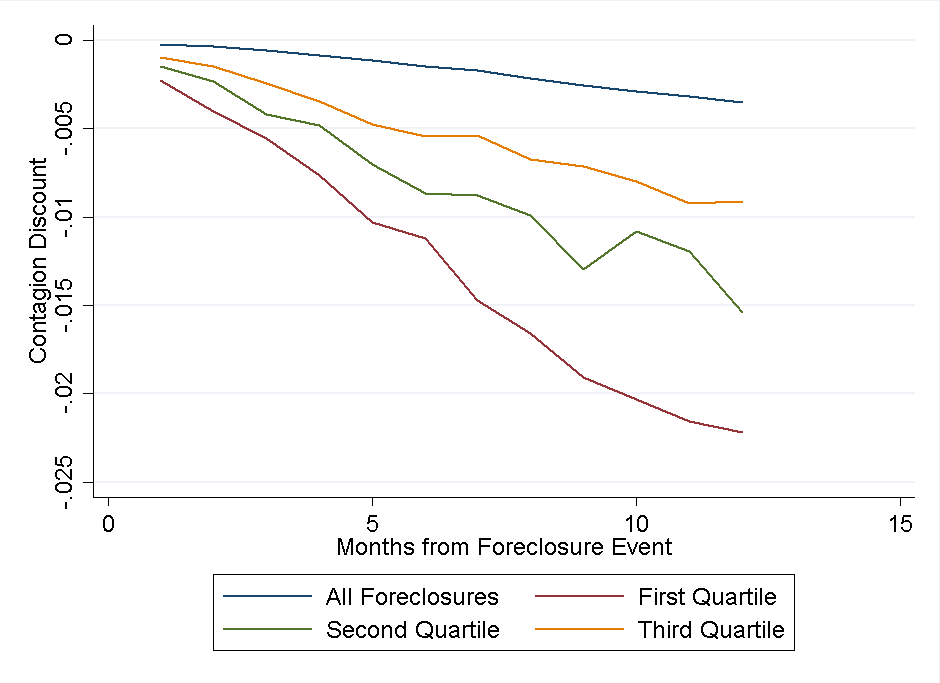
\includegraphics[width=\textwidth]{20MSA_nonlinquart.png}
\caption{\tiny Average non-linear contagion affect by quartile. The figure displays the estimated non-linear discount with heteroskedasticity-consistent standard errors originating from one foreclosure event per ten thousand home in a ZIP code by quartile. The time period ranges from $t+1$ to $t+12$. }
\end{figure}

While the literature is consistent in the non-linearity of foreclosure contagion, analysis of distance invariant foreclosure shows that the inclusion of non-linear terms does not significantly impact foreclosure discounts over time. Thus we conclude that foreclosure discounts behave linearly with time, but non-linearly with distance.

\subsection{Robustness}
In order to test our results for robustness, we employ the percentage of home sales in foreclosure as our foreclosure measurement and estimate our parameters. Because we believe foreclosure contagion to be linear as a function of time, we only estimate the linear model.

\import{Regs/}{Simple_Qt_results.tex}

\begin{figure}\label{fig:robust_lin} 
\centering
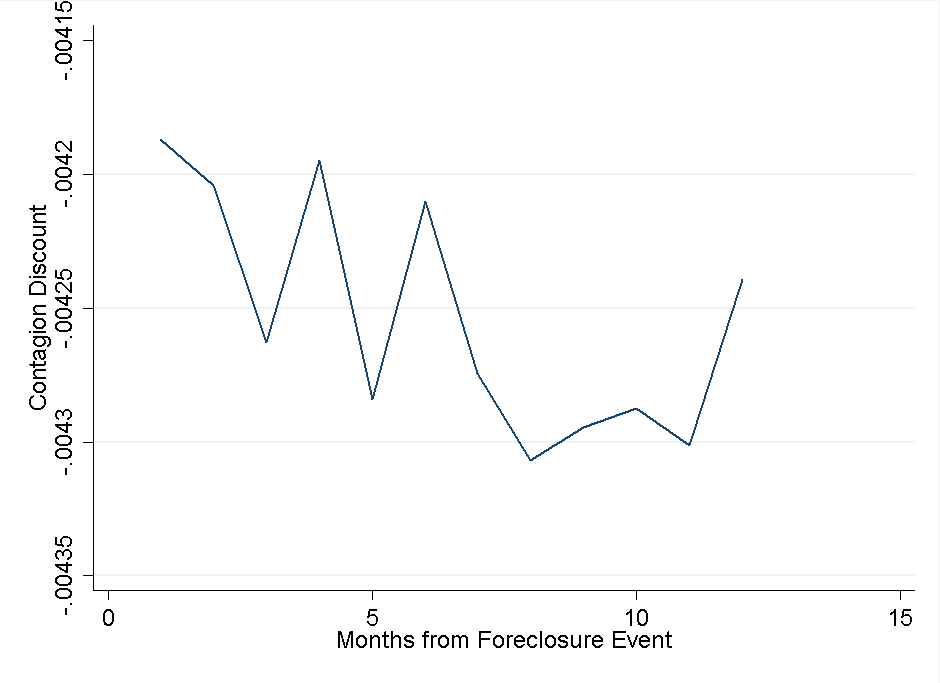
\includegraphics[width=\textwidth]{robust_20MSA_solo.png}
\caption{\tiny Average linear contagion affect using percentage home sales which were foreclosures. The figure displays the estimated average linear discount with heteroskedasticity-consistent standard errors originating from one foreclosure event per ten thousand home in a ZIP code. The time period ranges from $t+1$ to $t+12$. }
\end{figure}

Our results are consistent with the previous foreclosure variable. We this consider our model to be robust to a change in measurement variables. However, we also find that foreclosure contagion has a higher average variance. We hypothesize that this is the result of several factors. The first is that this percentage change of home sales in foreclosure does not measure foreclosure levels directly. Instead, it measures the number of foreclosed homes being sold. Considering that foreclosure can be a lengthy process, there may be a significant time lag between actual foreclosure rates and their reflection in the percentage of foreclosed homes being sold.

\section{Conclusion}
We use median home prices to provide joint estimates of national housing trends and foreclosure discount contagion. We find that housing prices are negatively impacted by foreclosures.Our analysis is novel in that we find that foreclosure discount contagion behaves linearly with time. We interpret these parameters as suggesting that foreclosure discount contagion is primarily the result of blight.

 The deluge of news articles and during the housing crises and subsequent surrounding the potential for strategic default highlights home owner sensitivity to changes in home value. Because foreclosure contagion behaves linearly, an increase in foreclosure rates will have a persistent impact on home prices across time. As a result, we feel that home owners should additionally be sensitive to an initial rise in foreclosure rates. 
 
 Our findings also have significant policy implications. Since the 2008 housing crises, there has been an increased interest in extending the capacity of foreclosure relief programs. In order to be effective, however, such programs must be able target areas where their intervention would be greatest. Our findings indicate that foreclosure relief efforts may have their highest rate of impact during the early stages of a housing crisis.
\newpage
\printbibliography


\newpage

\appendix
\section{Appendix} \label{app:B}
\import{Tables/}{HvAll.tex}
\import{Tables/}{Dfore.tex}
\import{Tables/}{Dfore_sq.tex}
\import{Tables/}{smaller_reg.tex}\label{tab:baseline}



\import{Metros/}{HV_1}
\import{Metros/}{HV_2}
\import{Metros/}{HV_3}




\end{document}


